\documentclass[xcolor=dvipsnames]{beamer}
\usepackage[utf8]{inputenc}
\usepackage{lmodern}
\usepackage[T1]{fontenc}
\usepackage{bm}
\usepackage{bigfoot} % to allow verbatim in footnote
\usepackage[numbered,framed]{matlab-prettifier}

\usepackage{xcolor}
\usepackage{mathtools}

\makeatletter
\newcommand{\redub}{}
\def\redub#1{%
  \@ifnextchar_%
    {\@redub{#1}}
    {\@latex@warning{Missing argument for \string\redub}\@redub{#1}_{}}%
}
\def\@redub#1_#2{%
    \colorlet{currentcolor}{.}%
    \color{red}%
    \underbrace{\color{currentcolor}#1}_{\color{red}#2}%
    \color{currentcolor}%
}
\makeatother

\newsavebox{\firstexample}
\newsavebox{\secondexample}
\usetheme{lankton-keynote}
\setbeamercolor{title}{fg=White}
\setbeamercolor{frametitle}{fg=White}
\let\ph\mlplaceholder % shorter macro
\lstMakeShortInline"
\lstset{
  style              = Matlab-editor,
  basicstyle         = \mlttfamily,
  escapechar         = ",
  mlshowsectionrules = true,
}

\author{Christopher Lillthors Viktor Kronvall}
\title{Pilbågen}

\begin{document}
\maketitle
\setbeamertemplate{frametitle}[default][center]

%define MATLAB-code boxes.
\begin{lrbox}{\firstexample}
\lstinputlisting[caption = {findroot.m}]{../Labb3/findroot.m}
\end{lrbox}

\begin{lrbox}{\secondexample}
\lstinputlisting[caption = {Sample code from Matlab}]{../Labb3/findroot.m}
\end{lrbox}

% slide 1
\begin{frame}
\frametitle{Problem}
%include the first box here.
% \usebox{\firstexample}
\begin{figure}[h!]
\centering
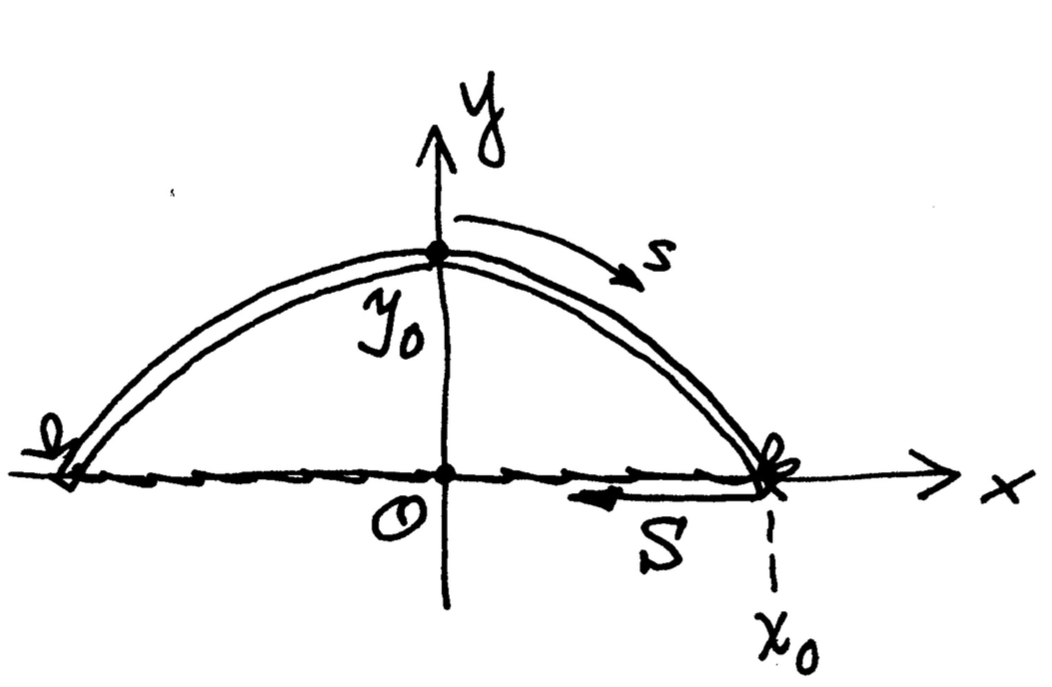
\includegraphics[scale=0.2]{bild.png}
\end{figure}
\end{frame}

% slide 2
\begin{frame}
\frametitle{Problem}
\begin{figure}[h!]
\centering
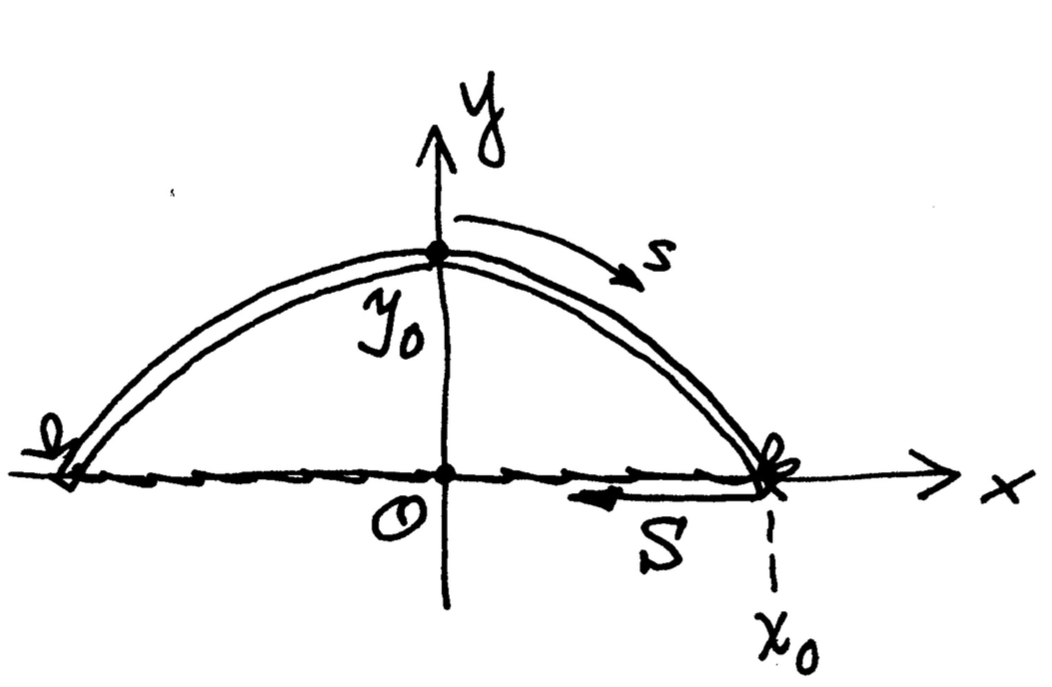
\includegraphics[scale=0.1]{bild.png}
\end{figure}
\begin{equation} \label{eq:original}
	\dfrac{d^2y}{dx^2} + qy \left(1+\left(\dfrac{dy}{dx}\right)^2\right)^{3/2} = 0 \nonumber
\end{equation}
\begin{equation}
s = \int_0^a{\sqrt{1+y'(x)^2}}=0.5 \nonumber
\end{equation}
\end{frame}

% slide 3
\begin{frame}
\frametitle{Problem}
\begin{figure}[h!]
\centering
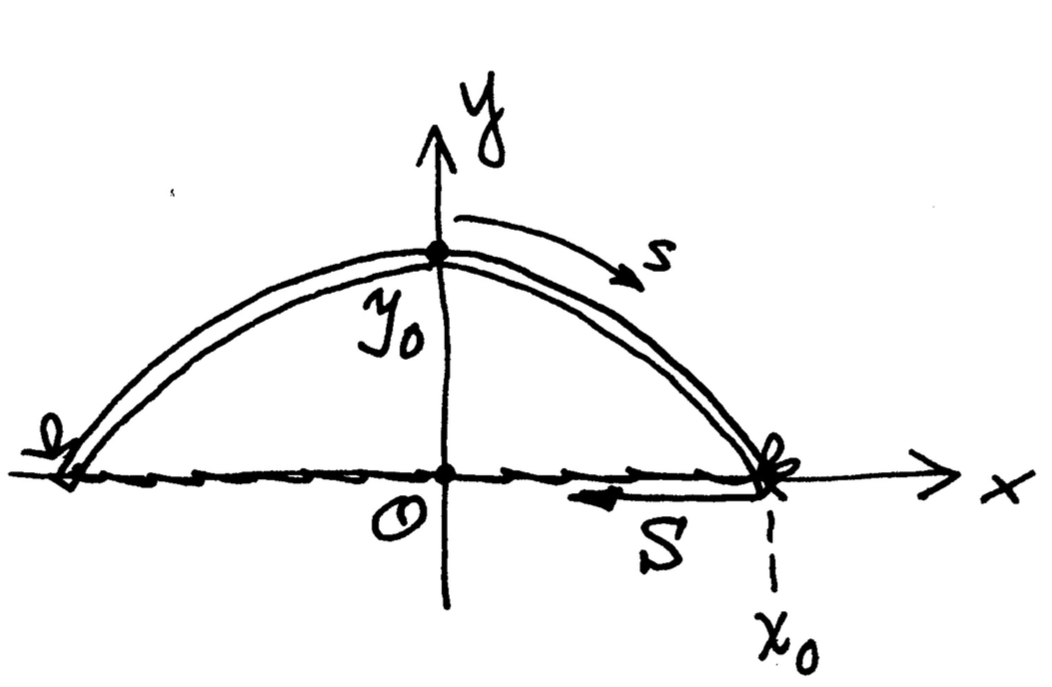
\includegraphics[scale=0.1]{bild.png}
\end{figure}
\begin{equation} \label{eq:original}
	\dfrac{d^2y}{dx^2} + qy \redub{\left(1+\left(\dfrac{dy}{dx}\right)^2\right)^{3/2}}_{\approx 1} = 0 \nonumber
\end{equation}
\begin{equation}
s = \int_0^a{\sqrt{1+y'(x)^2}}=0.5 \nonumber
\end{equation}
\end{frame}

% slide 4
\begin{frame}
\frametitle{Problem}
\begin{equation} \label{eq:simplified}
	\dfrac{d^2y}{dx^2} + qy = 0 \nonumber
\end{equation}
\begin{equation}
	y=e^{rx}
\end{equation}

\\
\begin{equation}
 y(x) = A cos(\sqrt{q}\:x)+B sin(\sqrt{q}\:x) \nonumber
\end{equation}
\begin{equation}
 y'(x) = -A\sqrt{q}\: sin(\sqrt{q}\:x) + B\sqrt{q}\:cos(\sqrt{q}\:x) \nonumber
\end{equation}
\end{frame}


\end{document}